\documentclass[11pt,a4paper]{article}

\usepackage[T1]{fontenc}
\usepackage[utf8]{inputenc}
\usepackage{lmodern}
\usepackage{microtype}
\usepackage[margin=2.6cm]{geometry}
\usepackage{amsmath,amssymb}
\usepackage{booktabs}
\usepackage{graphicx}
\usepackage{caption}
\usepackage{xcolor}
\usepackage[hidelinks]{hyperref}
\usepackage[numbers,sort&compress]{natbib}

\definecolor{fnblue}{HTML}{1F4FE0}
\hypersetup{colorlinks=true,linkcolor=fnblue,citecolor=fnblue,urlcolor=fnblue}
\captionsetup{font=small,labelfont=bf}
\graphicspath{{figures/}}

% generated by paper/make_assets.py, do not edit by hand
\newcommand{\BnStart}{February 2021}
\newcommand{\BnEnd}{May 2025}
\newcommand{\BnPeriods}{4{,}731}
\newcommand{\BnYears}{4.3}
\newcommand{\BnBaseSharpe}{1.32}
\newcommand{\BnBaseCagr}{42.3}
\newcommand{\BnBaseCarry}{10.2}
\newcommand{\BnBasePrice}{33.9}
\newcommand{\BnBasePvol}{30}
\newcommand{\BnBaseMaxDD}{\ensuremath{-}32.1}
\newcommand{\BnBaseCorr}{\ensuremath{-}0.04}
\newcommand{\BnASharpe}{1.46}
\newcommand{\BnACagr}{44.5}
\newcommand{\BnACarry}{9.6}
\newcommand{\BnAPrice}{35.8}
\newcommand{\BnAPvol}{28}
\newcommand{\BnAMaxDD}{\ensuremath{-}29.5}
\newcommand{\BnACorr}{\ensuremath{-}0.04}
\newcommand{\BnBSharpe}{1.28}
\newcommand{\BnBCagr}{38.6}
\newcommand{\BnBCarry}{10.0}
\newcommand{\BnBPrice}{31.7}
\newcommand{\BnBPvol}{29}
\newcommand{\BnBMaxDD}{\ensuremath{-}23.6}
\newcommand{\BnBCorr}{\ensuremath{-}0.04}
\newcommand{\BnCSharpe}{1.48}
\newcommand{\BnCCagr}{42.3}
\newcommand{\BnCCarry}{9.3}
\newcommand{\BnCPrice}{34.6}
\newcommand{\BnCPvol}{26}
\newcommand{\BnCMaxDD}{\ensuremath{-}20.5}
\newcommand{\BnCCorr}{\ensuremath{-}0.04}
\newcommand{\BnDSharpe}{1.41}
\newcommand{\BnDCagr}{39.4}
\newcommand{\BnDCarry}{9.3}
\newcommand{\BnDPrice}{34.0}
\newcommand{\BnDPvol}{26}
\newcommand{\BnDMaxDD}{\ensuremath{-}20.0}
\newcommand{\BnDCorr}{\ensuremath{-}0.03}
\newcommand{\BnCarrySharpe}{22.9}
\newcommand{\BnCarryVol}{0.45}
\newcommand{\BnCarryLong}{\ensuremath{-}1.7}
\newcommand{\BnCarryShort}{\ensuremath{+}14.6}
\newcommand{\BnCarryShareVar}{0.02}
\newcommand{\BnBestWinStart}{April 2021}
\newcommand{\BnBestWinEnd}{July 2021}
\newcommand{\BnBestWinPrice}{90}
\newcommand{\BnTotalPrice}{147}
\newcommand{\BnBestWinShare}{62}
\newcommand{\BnTopOneName}{SAND}
\newcommand{\BnTopOneContrib}{\ensuremath{+}16}
\newcommand{\BnTopTwoName}{AXS}
\newcommand{\BnTopTwoContrib}{\ensuremath{+}15}
\newcommand{\BnTopOneWeight}{0.020}
\newcommand{\BnWinNegNet}{29}
\newcommand{\BnWinNegPrice}{30}
\newcommand{\BnWinWorseLive}{3}
\newcommand{\ByStart}{August 2022}
\newcommand{\ByEnd}{May 2025}
\newcommand{\ByPeriods}{3{,}091}
\newcommand{\ByYears}{2.8}
\newcommand{\ByBaseSharpe}{1.24}
\newcommand{\ByBaseCagr}{32.3}
\newcommand{\ByBaseCarry}{7.1}
\newcommand{\ByBasePrice}{28.8}
\newcommand{\ByBasePvol}{25}
\newcommand{\ByBaseMaxDD}{\ensuremath{-}22.8}
\newcommand{\ByBaseCorr}{0.01}
\newcommand{\ByASharpe}{1.12}
\newcommand{\ByACagr}{26.7}
\newcommand{\ByACarry}{6.4}
\newcommand{\ByAPrice}{25.1}
\newcommand{\ByAPvol}{24}
\newcommand{\ByAMaxDD}{\ensuremath{-}19.1}
\newcommand{\ByACorr}{\ensuremath{-}0.01}
\newcommand{\ByBSharpe}{0.99}
\newcommand{\ByBCagr}{22.5}
\newcommand{\ByBCarry}{6.7}
\newcommand{\ByBPrice}{21.4}
\newcommand{\ByBPvol}{23}
\newcommand{\ByBMaxDD}{\ensuremath{-}21.6}
\newcommand{\ByBCorr}{0.01}
\newcommand{\ByCSharpe}{0.90}
\newcommand{\ByCCagr}{18.4}
\newcommand{\ByCCarry}{6.0}
\newcommand{\ByCPrice}{18.6}
\newcommand{\ByCPvol}{21}
\newcommand{\ByCMaxDD}{\ensuremath{-}20.7}
\newcommand{\ByCCorr}{\ensuremath{-}0.01}
\newcommand{\ByDSharpe}{0.79}
\newcommand{\ByDCagr}{15.5}
\newcommand{\ByDCarry}{6.0}
\newcommand{\ByDPrice}{17.7}
\newcommand{\ByDPvol}{21}
\newcommand{\ByDMaxDD}{\ensuremath{-}21.2}
\newcommand{\ByDCorr}{0.00}
\newcommand{\ByCarrySharpe}{11.2}
\newcommand{\ByCarryVol}{0.63}
\newcommand{\ByCarryLong}{\ensuremath{+}0.7}
\newcommand{\ByCarryShort}{\ensuremath{+}9.7}
\newcommand{\ByCarryShareVar}{0.06}
\newcommand{\ByBestWinStart}{November 2024}
\newcommand{\ByBestWinEnd}{February 2025}
\newcommand{\ByBestWinPrice}{63}
\newcommand{\ByTotalPrice}{81}
\newcommand{\ByBestWinShare}{78}
\newcommand{\ByTopOneName}{DOT}
\newcommand{\ByTopOneContrib}{\ensuremath{+}13}
\newcommand{\ByTopTwoName}{COMP}
\newcommand{\ByTopTwoContrib}{\ensuremath{+}10}
\newcommand{\ByTopOneWeight}{\ensuremath{-}0.036}
\newcommand{\ByWinNegNet}{23}
\newcommand{\ByWinNegPrice}{24}
\newcommand{\ByWinWorseLive}{0}
\newcommand{\LiveStart}{6 June 2026}
\newcommand{\LiveEnd}{6 November 2026}
\newcommand{\LiveDays}{153}
\newcommand{\LiveSteps}{130}
\newcommand{\LiveTotal}{\ensuremath{-}15.3}
\newcommand{\LiveLoss}{15.3}
\newcommand{\LiveEquity}{84{,}700}
\newcommand{\LiveCarry}{\ensuremath{+}2.50}
\newcommand{\LivePrice}{\ensuremath{-}17.31}
\newcommand{\LiveAnnRet}{\ensuremath{-}39.6}
\newcommand{\LiveAnnVol}{29}
\newcommand{\LiveSharpe}{\ensuremath{-}1.35}
\newcommand{\LiveCarryAnn}{6.0}
\newcommand{\LivePriceVol}{29}
\newcommand{\LiveStepPriceStd}{1.64}
\newcommand{\LiveStepCarryStd}{0.052}
\newcommand{\LiveStepRatio}{31}
\newcommand{\LiveWorstStep}{\ensuremath{-}9.53}
\newcommand{\LiveSecondWorst}{\ensuremath{-}8.14}
\newcommand{\LiveBestStep}{3.98}
\newcommand{\LiveBigSteps}{4}
\newcommand{\LiveSE}{2.05}
\newcommand{\LiveZ}{\ensuremath{-}1.26}
\newcommand{\LiveGaps}{1}
\newcommand{\LiveLongestGap}{23}
\newcommand{\LiveBetaBtc}{0.06}
\newcommand{\LiveRsqBtc}{1}
\newcommand{\LiveRsqBoth}{2}
\newcommand{\LiveWorstBtc}{\ensuremath{+}10.1}
\newcommand{\LiveSecondBtc}{\ensuremath{-}1.8}
\newcommand{\LiveWorstDate}{21 September}
\newcommand{\LiveSecondDate}{9 September}
\newcommand{\BnWinWorseClean}{19}
\newcommand{\ByWinWorseClean}{14}
\newcommand{\CleanSteps}{458}
\newcommand{\CleanRebs}{21}
\newcommand{\RealRebs}{16}
\newcommand{\CleanTotal}{\ensuremath{-}4.8}
\newcommand{\CleanLoss}{4.8}
\newcommand{\CleanCarry}{\ensuremath{+}1.46}
\newcommand{\CleanPrice}{\ensuremath{-}5.13}
\newcommand{\CleanCarryAnn}{3.5}
\newcommand{\CleanSharpe}{\ensuremath{-}0.49}
\newcommand{\CleanZ}{\ensuremath{-}0.84}
\newcommand{\CleanPriceVol}{24}
\newcommand{\CleanRsqBtc}{1}
\newcommand{\CleanGap}{10.5}
\newcommand{\CleanEnd}{6 November, 08:00}
\newcommand{\OctCarryReal}{\ensuremath{+}1.43}
\newcommand{\OctCarryClean}{\ensuremath{+}0.46}
\newcommand{\LongOverlap}{5}
\newcommand{\LongSize}{10}


\title{\textbf{Carry or Dispersion?}\\[0.3em]
\large A live post-mortem of a beta-hedged funding book on crypto perpetuals}
\author{Noa Robles Levy\\[0.2em]
\small Fractal North Research}
\date{\small Working paper, November 2026. Revised 7 November 2026.}

\begin{document}
\maketitle

\begin{abstract}
\noindent
A cross-sectional funding-carry book on 23 crypto perpetual futures goes long the
eleven coins with the lowest funding rate, short the eleven with the highest, and
hedges its net beta to BTC. In backtests it earns a Sharpe ratio of about
\BnBaseSharpe{} (Binance, \BnStart{} to \BnEnd) and \ByBaseSharpe{} (Bybit,
\ByStart{} to \ByEnd). Run as a live shadow ledger on Bybit for \LiveDays{} days, it
lost \LiveLoss\%. That ledger only advanced while its host machine was on, so it
rebalanced irregularly; replaying the same period on the intended schedule (every
seven days) gives a loss of \CleanLoss\% instead. Rebalance timing alone moved a
five-month result by \CleanGap{} points, because it changed which coins were held. I
decompose every period's profit and loss into a funding (carry) leg and a price leg.
In both versions the carry was positive and steady but modest (\CleanCarryAnn\% a
year on the clean schedule, against \ByBaseCarry\% in the Bybit backtest), and the
result was decided by the price leg, which is not a hedging failure in the usual sense:
its $R^2$ against BTC is \LiveRsqBtc\% in both. The price leg is a cross-sectional
dispersion bet. It carries more than 99.9\% of the book's variance in backtests, earns
most of its historical return in a single 90-day window, and is not removed by
refinements such as inverse-volatility weighting or a second (ETH) hedge factor, whose
effect on the Sharpe ratio flips sign between venues. On the clean schedule the live
result is unremarkable relative to the backtest ($z=\CleanZ$). The constructive finding
is that nearly all of the carry comes from the short leg, which points to a per-coin
delta-neutral construction as the way to isolate it.
\end{abstract}

\section{Introduction}

Funding on perpetual futures is one of the few cash flows in crypto markets that is
paid on a fixed schedule regardless of direction. A position that is short when
funding is positive is paid every eight hours. A natural way to collect it
systematically is a cross-sectional book: short the coins whose funding is highest,
long the coins whose funding is lowest, and receive the spread. This is the crypto
analogue of the carry trades documented across asset classes by
\citet{koijen2018carry}.

The difficulty is that high funding is not random. It marks coins that leveraged
traders are crowding into, which are typically the most volatile coins with the
strongest recent momentum. Shorting them imports a large price exposure. The usual
answer is a beta hedge to BTC. The book studied here does exactly that, and its
backtest looked attractive: a Sharpe ratio above one on two venues, with a carry leg
that on its own is almost riskless.

The recorded live result was a loss of \LiveLoss\% in \LiveDays{} days; on the
schedule the strategy actually specifies, the same period gives \CleanTotal\%. This
paper asks why the book lost money, and why the rebalance schedule mattered so much.
The answer to both is not that the carry failed, nor that the hedge was mis-specified,
but that the book was never mainly a carry strategy. Its risk, and most of its historical
return, sit in a residual price leg that is orthogonal to BTC and ETH and driven by
the dispersion of individual coins around the market.

The contribution is a careful decomposition rather than a new signal. Section~\ref{sec:setup}
describes the strategy and data. Section~\ref{sec:live} reports the live ledger and
shows that its losses are unrelated to BTC. Section~\ref{sec:backtest} shows that the
same structure is present in backtests, and that the price leg's historical return is
concentrated in a few episodes. Section~\ref{sec:variants} tests whether better weights
or a second hedge factor fix the problem. Section~\ref{sec:discussion} discusses what
the evidence does and does not support, and what to build next.

\section{Strategy and data}\label{sec:setup}

\subsection{Funding mechanics}

A perpetual future has no expiry. To keep its price close to spot, longs and shorts
exchange a funding payment at fixed times (every eight hours on both venues used
here). With position weight $w_i$ (fraction of equity, positive for long) and funding
rate $f_{i,t}$, the funding P\&L over period $t$ is $-w_i f_{i,t}$: when funding is
positive, longs pay and shorts receive.

\subsection{Book construction}

The universe is 23 liquid USDT-margined perpetuals.\footnote{BTC, ETH, BNB, XRP, ADA,
SOL, DOGE, LINK, DOT, LTC, BCH, FIL, NEAR, AVAX, XLM, AAVE, UNI, TRX, ATOM, ETC, SAND,
AXS, COMP.} At each rebalance, every seven days, coins are ranked on their latest
funding rate. With $L_t$ the $N=11$ lowest and $S_t$ the $N=11$ highest,
\begin{equation}
  w_{i,t} =
  \begin{cases}
    +1/N & i \in L_t,\\
    -1/N & i \in S_t,\\
    0 & \text{otherwise,}
  \end{cases}
\end{equation}
so each leg has a gross exposure of one and the book is dollar-neutral before
hedging. Its funding income is the cross-sectional spread
$\tfrac{1}{N}\big(\sum_{i\in S_t} f_{i,t} - \sum_{i\in L_t} f_{i,t}\big)$.

The hedge is written generally. Let $F$ be a set of hedge instruments with return
vector $\mathbf{F}_t$ and trailing covariance matrix $\Sigma_F$, estimated over 90
eight-hour periods (30 days). The book's exposure to factor $k$ is
$e_k = \sum_i w_i \operatorname{Cov}(r_i, F_k)$, and the hedge that makes the book
jointly neutral to all factors is
\begin{equation}\label{eq:hedge}
  \mathbf{h} = -\Sigma_F^{-1}\,\mathbf{e}.
\end{equation}
With $F=\{\text{BTC}\}$ this reduces to the familiar single-beta hedge
$h = -\sum_i w_i \beta_i$, which is the live configuration. Using the inverse of
$\Sigma_F$ rather than separate betas matters when factors are correlated, as BTC and
ETH are: two separate hedges would remove their common component twice.

\subsection{P\&L decomposition}

Every period's return is split into
\begin{equation}
  \pi_t = \underbrace{\textstyle\sum_i -w_i f_{i,t} - \sum_k h_k f_{k,t}}_{\text{carry}}
        + \underbrace{\textstyle\sum_i w_i r_{i,t} + \sum_k h_k F_{k,t}}_{\text{price}}
        - \text{cost}_t ,
\end{equation}
with costs of 8 basis points on the turnover of both legs and hedge. Ranks, betas and
volatilities at $t$ use information up to $t-1$; P\&L is realised over $t \to t+1$.

\subsection{Data}

Backtests use two venues. \emph{Binance}: hourly closes and funding for all 23 coins,
\BnStart{} to \BnEnd{} (\BnPeriods{} eight-hour periods, \BnYears{} years).
\emph{Bybit}, the venue of the live test: \ByStart{} to \ByEnd{} (\ByPeriods{}
periods, \ByYears{} years). Every variant starts trading only after a 35-day warm-up,
so that all variants are evaluated on exactly the same periods.\footnote{An earlier
version of this comparison let the inverse-volatility variants sit flat during the
first week of January 2021, an extreme week for altcoins, while the baseline traded
it. That flattered them by about 0.13 Sharpe. The warm-up removes the asymmetry.}

The live test is a \emph{shadow ledger}: no orders are sent. A scheduled job pulls
live Bybit prices and the funding events that actually printed, marks the book to
market, accrues funding, and rebalances every seven days. It ran from \LiveStart{} to
\LiveEnd{} (\LiveSteps{} steps). Because the data did not exist when the strategy was
fixed, this is a genuine out-of-sample test of both the price behaviour and the
assumption that funding accrues as modelled. One implementation detail turned out to
matter: the job only ran while its host machine was on, so steps were irregular (from
minutes to \LiveLongestGap{} days apart) and rebalances happened whenever the job next
ran after seven days had passed. Section~\ref{sec:schedule} quantifies the effect by
replaying the same period on the intended schedule.

\section{The live ledger}\label{sec:live}

\begin{figure}[t]
  \centering
  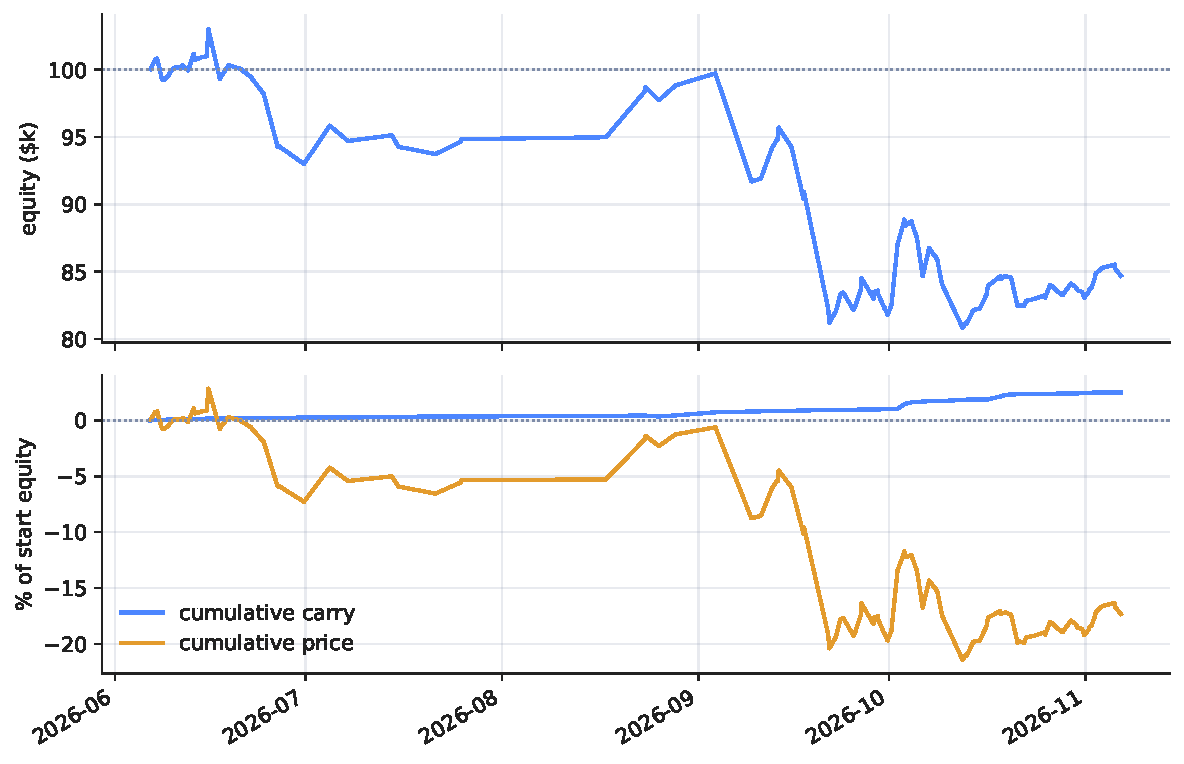
\includegraphics[width=0.9\linewidth]{live_ledger.pdf}
  \caption{Live shadow ledger on Bybit, \LiveStart{} to \LiveEnd. Top: equity of the
  unlevered book. Bottom: cumulative carry and price contributions. Carry rises
  steadily; the price leg determines the outcome.}
  \label{fig:live}
\end{figure}

Table~\ref{tab:live} and Figure~\ref{fig:live} summarise the live result. Equity fell
from \$100{,}000 to \$\LiveEquity. The carry leg contributed \LiveCarry\% and the price
leg \LivePrice\%.

\begin{table}[h]
  \centering
  \small
  \begin{tabular}{lr}
    \toprule
    Days live / steps & \LiveDays{} / \LiveSteps \\
    Cumulative return & \LiveTotal\% \\
    \quad of which carry & \LiveCarry\% \\
    \quad of which price & \LivePrice\% \\
    Annualised log return & \LiveAnnRet\% \\
    Annualised volatility & \LiveAnnVol\% \\
    Sharpe ratio (time-normalised) & \LiveSharpe \\
    Carry, annualised (Bybit backtest: \ByBaseCarry\%) & \LiveCarryAnn\% \\
    Std.\ of price P\&L per step & \LiveStepPriceStd\% \\
    Std.\ of carry P\&L per step & \LiveStepCarryStd\% \\
    Worst / best price step & \LiveWorstStep\% / \LiveBestStep\% \\
    \bottomrule
  \end{tabular}
  \caption{Live summary. Steps are irregular, from minutes to \LiveLongestGap{} days
  apart, so annualised figures use time-normalised estimators: return
  $\sum_j \ell_j / T$ and volatility $\sqrt{\sum_j \ell_j^2 / T}$, with $\ell_j$ the log
  return of step $j$ and $T$ the elapsed time in years.}
  \label{tab:live}
\end{table}

\paragraph{The carry was positive, but modest.} Recorded funding income annualised to
\LiveCarryAnn\%, close to the \ByBaseCarry\% the same configuration earned in the Bybit
backtest. That comparison flatters the carry: on the clean schedule of
Section~\ref{sec:schedule} it annualises to \CleanCarryAnn\%, about half the backtest
rate. The two ledgers earn nearly the same carry in every month except October
(\OctCarryReal\% recorded against \OctCarryClean\% clean), when the recorded book
happened to hold coins with unusually high funding. The cash flow is real and accrues
as modelled, but it is smaller than the backtest suggested.\footnote{The live script
quotes a higher expectation (9.2\%) taken from an earlier research notebook with a
different sample.}

\paragraph{The price leg dominated.} Per step, the price P\&L was \LiveStepRatio{}
times more volatile than the carry P\&L. There were \LiveBigSteps{} steps with a price
move above 4\%, the worst at \LiveWorstStep\% and \LiveSecondWorst\%. A book that is
genuinely market-neutral should not produce such steps.

\paragraph{It was not BTC.} The obvious suspect is a hedge that failed to neutralise
the market. Regressing each step's price P\&L on the BTC log return over the same
interval (Figure~\ref{fig:scatter}) gives a slope of \LiveBetaBtc{} and an $R^2$ of
\LiveRsqBtc\%. Adding ETH raises the $R^2$ to \LiveRsqBoth\%. The worst step, ending
\LiveWorstDate, coincided with a BTC move of \LiveWorstBtc\%: the beta hedge gained,
but the shorted high-funding coins rallied much harder. The second worst, ending
\LiveSecondDate, came with BTC at only \LiveSecondBtc\%. The hedge did its job. What
remained is the dispersion of individual coins around the market, which a hedge in
BTC, or in BTC and ETH, cannot touch by construction.

\begin{figure}[t]
  \centering
  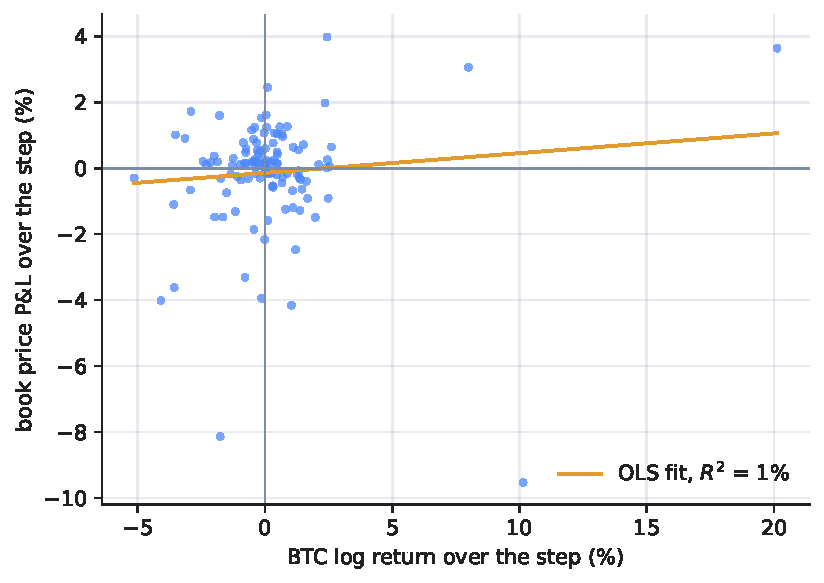
\includegraphics[width=0.62\linewidth]{live_btc_scatter.pdf}
  \caption{Live price P\&L per step against the BTC return over the same interval.
  The beta hedge works ($\beta\approx\LiveBetaBtc$); the large losses are unrelated
  to the market.}
  \label{fig:scatter}
\end{figure}

\subsection{How much did the schedule matter?}\label{sec:schedule}

The live ledger rebalanced \RealRebs{} times at irregular moments; the strategy
specifies a rebalance every seven days. Because the ledger is a shadow book, the
intended schedule can be reconstructed exactly from Bybit's public history: every
eight-hour funding time is marked to the close of the hour ending then, funding printed
in the interval is accrued, and the book is rebalanced every seven days using only
data available at that moment.\footnote{The replay uses the same weighting code as the
live job and was tested for two properties: running it in one pass or in several passes
with gaps gives identical ledgers, and the weights at a rebalance are identical whether
or not data after that moment is supplied.} Since 7 November 2026 the live job itself
works this way, so missed runs are caught up and no longer change the result.

\begin{table}[h]
  \centering
  \small
  \begin{tabular}{lrr}
    \toprule
    & Recorded ledger & Clean schedule \\
    \midrule
    Rebalances & \RealRebs & \CleanRebs \\
    Cumulative return & \LiveTotal\% & \CleanTotal\% \\
    \quad of which carry & \LiveCarry\% & \CleanCarry\% \\
    \quad of which price & \LivePrice\% & \CleanPrice\% \\
    Carry, annualised & \LiveCarryAnn\% & \CleanCarryAnn\% \\
    Sharpe ratio & \LiveSharpe & \CleanSharpe \\
    Price P\&L $R^2$ against BTC & \LiveRsqBtc\% & \CleanRsqBtc\% \\
    \bottomrule
  \end{tabular}
  \caption{Recorded live ledger against the same period replayed on the intended
  schedule (clean replay to \CleanEnd{} UTC, the last eight-hour mark before the end of
  the recorded window).}
  \label{tab:schedule}
\end{table}

\begin{figure}[t]
  \centering
  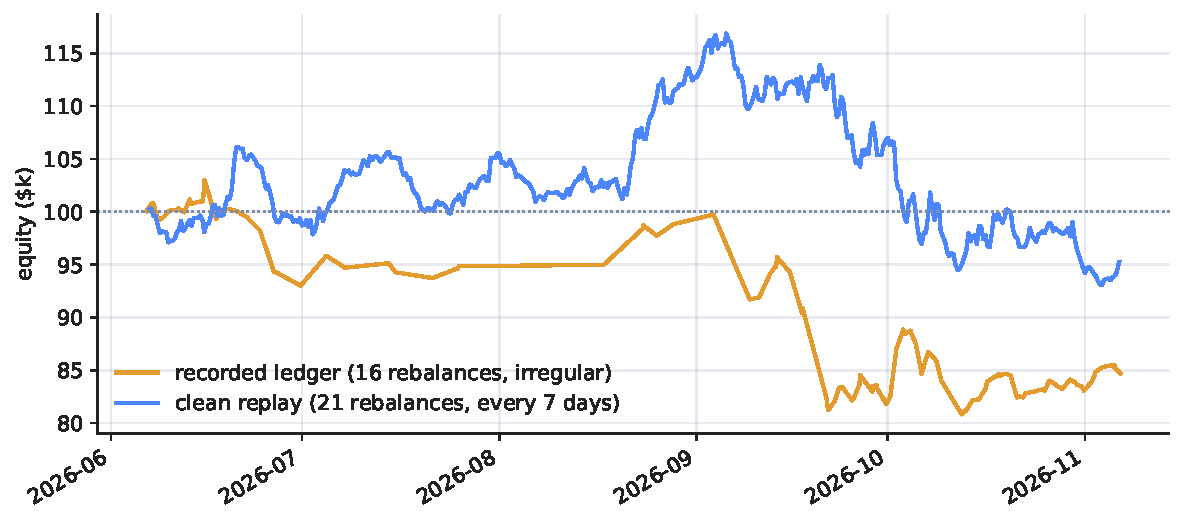
\includegraphics[width=0.9\linewidth]{live_clean_vs_recorded.pdf}
  \caption{The same strategy over the same period, rebalanced at irregular moments
  (recorded) and every seven days (clean). The paths separate at rebalances, when the
  two books start holding different coins.}
  \label{fig:schedule}
\end{figure}

Table~\ref{tab:schedule} and Figure~\ref{fig:schedule} show that the schedule moved the
five-month result by \CleanGap{} points. Nothing about the strategy's rules changed;
only the days on which it re-ranked the coins. Rebalancing on a different day selects
different coins: at the end of the window only \LongOverlap{} of the \LongSize{} long
positions (excluding BTC) are the same in the two books. In a book whose outcome is
decided by which coins are held during a few large dispersion moves, that is enough to
turn \CleanTotal\% into \LiveTotal\%. The sensitivity is itself evidence for the
paper's thesis: a carry strategy would barely notice the rebalance day; a dispersion
bet does. The diagnosis of the previous paragraphs is unaffected: on the clean schedule
too, the price leg dominates and is unrelated to BTC.

\paragraph{Is the loss significant?} Under i.i.d.\ returns the standard error of an
annualised Sharpe ratio estimated over $T$ years is approximately
$\sqrt{(1+\mathrm{SR}^2/2)/T}$ \citep{lo2002statistics}. With $T = \LiveDays/365$
and the Bybit backtest Sharpe of \ByBaseSharpe{} as the null, the standard error is
\LiveSE. The recorded Sharpe of \LiveSharpe{} gives $z = \LiveZ$; the clean schedule's
\CleanSharpe{} gives $z = \CleanZ$. Neither rejects the backtest. The empirical
distribution makes the role of the schedule sharper. Of all 153-day windows in the
backtests, \BnWinNegNet\% (Binance) and \ByWinNegNet\% (Bybit) lost money. A loss of
\LiveLoss\% or more, as recorded, occurred in only \BnWinWorseLive\% of Binance windows
and in none of the Bybit windows. A result of \CleanTotal\% or worse, as on the clean
schedule, occurred in \BnWinWorseClean\% and \ByWinWorseClean\% of windows. The
recorded loss lies beyond anything the backtest produced; the strategy as specified had
an ordinary bad five months. Most of what looked like a tail event was the execution
schedule.

\section{The same structure in backtests}\label{sec:backtest}

\begin{figure}[t]
  \centering
  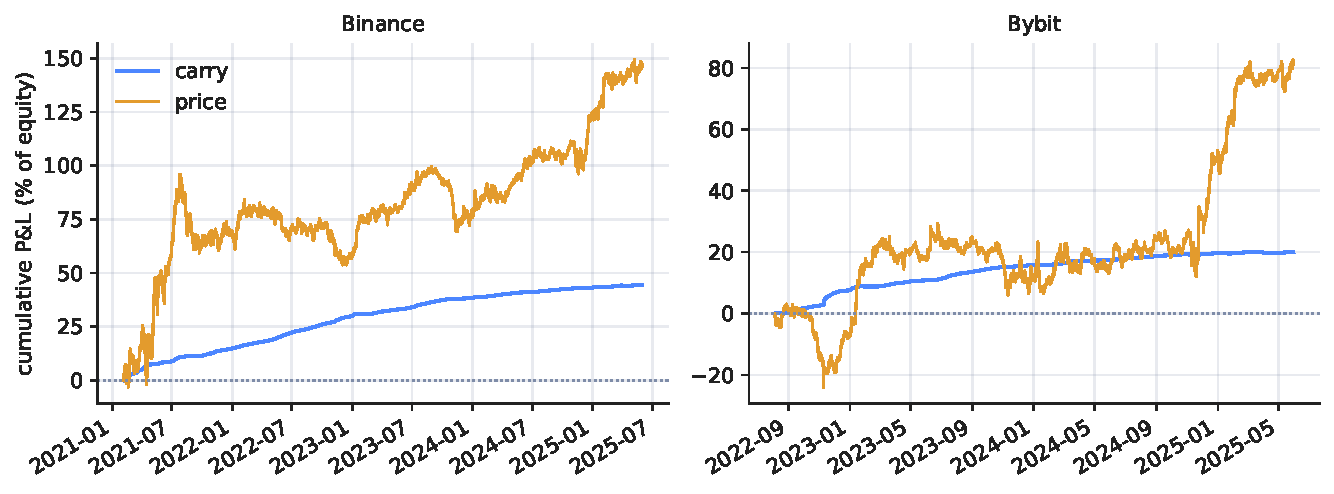
\includegraphics[width=\linewidth]{backtest_legs.pdf}
  \caption{Baseline book, cumulative carry and price contributions in the backtests.
  The carry is a straight line; the price leg has the shape of a volatile directional
  strategy whose gains arrive in bursts.}
  \label{fig:legs}
\end{figure}

Figure~\ref{fig:legs} shows that the live pattern is not new. In both backtests the
carry leg is close to a straight line: on its own it has a Sharpe ratio of
\BnCarrySharpe{} on Binance and \ByCarrySharpe{} on Bybit, with annualised volatility
below 1\%.\footnote{These carry Sharpe ratios overstate what is attainable. Funding
rates are persistent, so eight-hour carry returns are strongly autocorrelated and the
$\sqrt{1095}$ annualisation assumes independence. The qualitative point, that the carry
is nearly riskless relative to the price leg, survives any reasonable correction.} The
price leg, by contrast, has an annualised volatility of \BnBasePvol\% (Binance) and
\ByBasePvol\% (Bybit). The carry leg accounts for \BnCarryShareVar\% and
\ByCarryShareVar\% of the variance of net returns; the price leg accounts for the rest.

The backtests nonetheless look attractive because the price leg was \emph{profitable}:
\BnBasePrice\% a year on Binance and \ByBasePrice\% on Bybit, roughly three times the
carry. Its correlation with BTC is \BnBaseCorr{} and \ByBaseCorr{}, so like the live
losses these gains are pure dispersion: coins with low funding outperformed coins with
high funding, after removing the market.

\begin{table}[h]
  \centering
  \small
  \resizebox{\linewidth}{!}{%
  \begin{tabular}{lcc}
    \toprule
    & Binance & Bybit \\
    \midrule
    Total price P\&L, baseline & \BnTotalPrice\% & \ByTotalPrice\% \\
    Best 90-day window & \BnBestWinStart{} to \BnBestWinEnd & \ByBestWinStart{} to \ByBestWinEnd \\
    Price P\&L in that window & \BnBestWinPrice\% & \ByBestWinPrice\% \\
    Share of total & \BnBestWinShare\% & \ByBestWinShare\% \\
    Largest contributors in that window & \BnTopOneName{} (\BnTopOneContrib\%), \BnTopTwoName{} (\BnTopTwoContrib\%)
      & \ByTopOneName{} (\ByTopOneContrib\%), \ByTopTwoName{} (\ByTopTwoContrib\%) \\
    \bottomrule
  \end{tabular}}
  \caption{Concentration of the price leg's backtest return. Contributions are
  cumulative $\sum_t w_{i,t-1} r_{i,t}$ over the window, in percent of equity.}
  \label{tab:conc}
\end{table}

That return is concentrated in time (Table~\ref{tab:conc}). On Bybit, the best 90 days
(\ByBestWinStart{} to \ByBestWinEnd) delivered \ByBestWinShare\% of the price leg's
entire profit over almost three years; on Binance, \BnBestWinStart{} to
\BnBestWinEnd{} delivered \BnBestWinShare\%. Within those windows a handful of coins
dominate. Outside them the price leg earns far less, with large swings. A backtest
whose return depends this much on two or three episodes has a sampling error much
larger than its Sharpe ratio suggests, and a live window that contains no such episode
should be expected to do much worse than the backtest average.

There is an economic story under which the dispersion return is a premium rather than
luck. High funding marks crowded leveraged longs, and crowded positions tend to unwind,
so high-funding coins may underperform on average. The data here are too short and too
concentrated to distinguish that premium from a few fortunate episodes, and I do not
claim either.

\section{Do better weights or a second factor help?}\label{sec:variants}

If the problem is residual risk, two refinements suggest themselves. \emph{Inverse
volatility weighting}: within each leg, $w_i \propto 1/\sigma_i$ with $\sigma_i$ the
trailing 10-day volatility, normalised to a gross of one per leg. Under equal weights
the short leg, made of the most volatile coins, dominates the book's risk; inverse
volatility equalises the per-name risk contributions in the spirit of risk parity
\citep{maillard2010properties}. \emph{A second hedge factor}: ETH in addition to BTC,
using equation~\eqref{eq:hedge}. I also test re-hedging every period instead of only
at rebalance.

\begin{table}[t]
  \centering
  \small
  \setlength{\tabcolsep}{4.5pt}
  \resizebox{\linewidth}{!}{%
  \begin{tabular}{l rrrrr c rrrrr}
    \toprule
    & \multicolumn{5}{c}{Binance, \BnStart{} to \BnEnd} && \multicolumn{5}{c}{Bybit, \ByStart{} to \ByEnd} \\
    \cmidrule{2-6}\cmidrule{8-12}
    Variant & SR & CAGR & Carry & P.\,vol & MDD && SR & CAGR & Carry & P.\,vol & MDD \\
    \midrule
    Baseline: $1/N$, BTC & \BnBaseSharpe & \BnBaseCagr & \BnBaseCarry & \BnBasePvol & \BnBaseMaxDD
      && \ByBaseSharpe & \ByBaseCagr & \ByBaseCarry & \ByBasePvol & \ByBaseMaxDD \\
    A: inv.\ vol, BTC & \BnASharpe & \BnACagr & \BnACarry & \BnAPvol & \BnAMaxDD
      && \ByASharpe & \ByACagr & \ByACarry & \ByAPvol & \ByAMaxDD \\
    B: $1/N$, BTC+ETH & \BnBSharpe & \BnBCagr & \BnBCarry & \BnBPvol & \BnBMaxDD
      && \ByBSharpe & \ByBCagr & \ByBCarry & \ByBPvol & \ByBMaxDD \\
    C: inv.\ vol, BTC+ETH & \BnCSharpe & \BnCCagr & \BnCCarry & \BnCPvol & \BnCMaxDD
      && \ByCSharpe & \ByCCagr & \ByCCarry & \ByCPvol & \ByCMaxDD \\
    D: C, re-hedged each period & \BnDSharpe & \BnDCagr & \BnDCarry & \BnDPvol & \BnDMaxDD
      && \ByDSharpe & \ByDCagr & \ByDCarry & \ByDPvol & \ByDMaxDD \\
    \bottomrule
  \end{tabular}}
  \caption{Weighting and hedge variants. SR: annualised Sharpe ratio. CAGR, carry
  (annualised), price-leg volatility and maximum drawdown in percent. All variants
  trade the same periods after a 35-day warm-up, with 8 bps costs on turnover.}
  \label{tab:variants}
\end{table}

Table~\ref{tab:variants} and Figure~\ref{fig:variants} give the results. Two patterns
hold on both venues. Every refinement lowers the price-leg volatility (from
\BnBasePvol\% to \BnCPvol\% on Binance and from \ByBasePvol\% to \ByCPvol\% on Bybit
for variant C) and lowers the maximum drawdown. Re-hedging every period never improves
the Sharpe ratio: the weekly hedge is not stale, and the extra turnover costs more than
it saves.

The effect on the Sharpe ratio, however, flips sign. On Binance, variant C improves it
from \BnBaseSharpe{} to \BnCSharpe. On Bybit, the venue of the live test, it falls from
\ByBaseSharpe{} to \ByCSharpe, and each refinement makes it worse. The reason is
visible in the price column of Table~\ref{tab:variants}: the refinements reduce the
book's dispersion exposure, and whether that raises or lowers the Sharpe ratio depends
on whether the removed exposure happened to be profitable in that sample. They also
cannot remove much of it. Neither BTC nor ETH spans the idiosyncratic moves of the
other 21 coins, which is why the price-leg volatility falls by only 13 to 16\%.

With five variants tested on two samples, a Sharpe gain of 0.16 on one venue and a loss
of 0.34 on the other is not evidence of an improvement in expected return. It is
evidence of a modest reduction in risk. Selecting the variant that looks best in one
sample would be a textbook instance of the selection bias that deflated Sharpe ratios
are designed to catch \citep{bailey2014deflated,harvey2016cross}.

\begin{figure}[t]
  \centering
  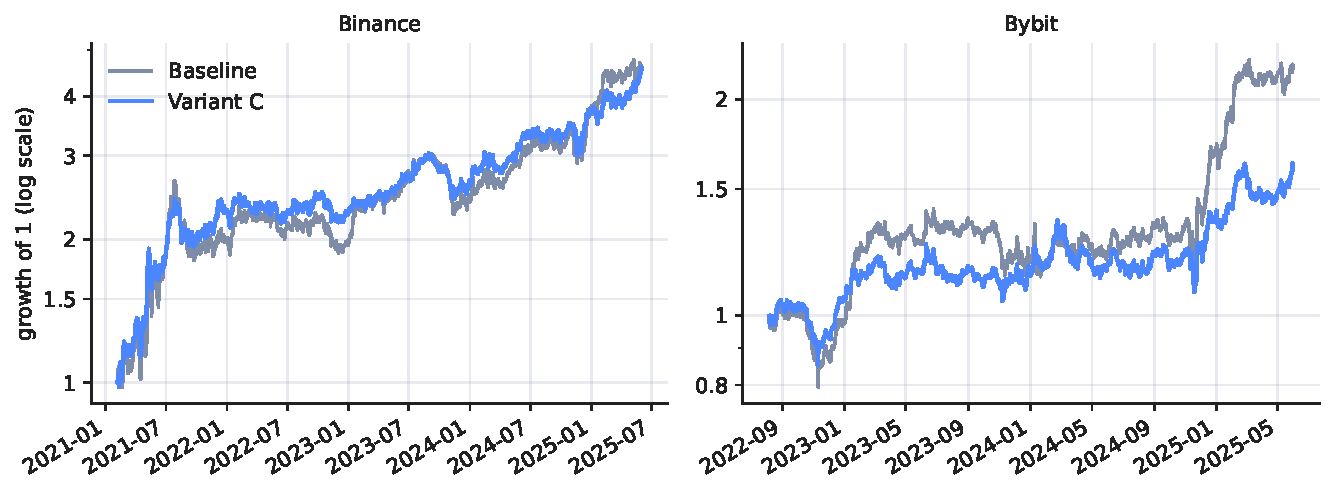
\includegraphics[width=\linewidth]{variants_equity.pdf}
  \caption{Growth of one unit, baseline versus variant C. Variant C is smoother on both
  venues; it ends higher on Binance and lower on Bybit.}
  \label{fig:variants}
\end{figure}

\section{Discussion}\label{sec:discussion}

\subsection{What the evidence supports}

The book should be described as what it is: a cross-sectional dispersion strategy with
a carry tailwind, not a carry strategy with residual risk. Its backtest Sharpe ratio of
\ByBaseSharpe{} to \BnBaseSharpe{} is earned by a price leg with 25 to 30\% volatility,
whose return is concentrated in a few episodes and so sensitive to which coins are
held that the rebalance day alone moved five months of live results by \CleanGap{}
points. On the intended schedule the live period was an ordinary bad stretch, not
evidence against the backtest; five months cannot settle whether the edge is real.
What the evidence does settle is that the strategy should not be run as a low-risk
carry product, and that its live carry ran at about half the backtest rate.

\subsection{Where the carry actually comes from}

Splitting the carry by leg (baseline) is the most useful number in this study. On
Binance the short leg earned \BnCarryShort\% a year and the long leg \BnCarryLong\%; on
Bybit, \ByCarryShort\% and \ByCarryLong\%. The long leg contributes nothing to the carry.
It is in the book only to offset the short leg's price exposure, and it does so poorly
because the long and short coins are different coins.

This suggests a different construction. Shorting the high-funding perpetuals and
holding the \emph{same} coins on spot (the classic cash-and-carry trade) collects the
short-leg funding while making each position delta-neutral by construction. The price
leg then reduces to the spot-perpetual basis of the same coin, which is far smaller
than the dispersion between different coins. This removes the dispersion bet instead
of trying to hedge it with market factors. It also has costs that the cross-sectional
book avoids: spot capital and custody, two venues or account types, and basis risk
around funding resets. I have not tested it here; it is the next experiment.

\subsection{Limitations}

\begin{itemize}
  \item \emph{Short samples.} 4.3 and 2.8 years of backtest, and five months live. The
    backtest results are dominated by a few episodes, so their sampling error is larger
    than the Sharpe ratios suggest.
  \item \emph{Shadow ledger, not fills.} The live test marks to last prices and charges
    no transaction costs at all; the backtests charge 8 bps on turnover. Real execution
    in the smaller coins would add costs and slippage, so the live figures are if
    anything optimistic.
  \item \emph{Execution schedule.} The recorded ledger only advanced while its host
    machine was on (the longest gap was \LiveLongestGap{} days), so it rebalanced at
    irregular moments. Section~\ref{sec:schedule} shows this moved the result by
    \CleanGap{} points. The clean replay is the better estimate of the strategy as
    specified, but it was reconstructed after the fact rather than recorded in real
    time; no rule or parameter was changed to produce it. From 7 November 2026 the live
    job replays missed steps itself.
  \item \emph{Fixed universe.} The 23 coins were chosen with hindsight, from coins that
    are still liquid today. That is survivorship bias in the backtest, which would
    flatter it.
  \item \emph{Multiple testing.} The variants were chosen after seeing the live losses.
    Section~\ref{sec:variants} reports all of them on both venues for that reason.
\end{itemize}

\subsection{Ongoing}

Variant C now runs live as a second, parallel shadow ledger from \LiveEnd{}, while the
baseline continues unchanged as a control; both now follow the clean schedule. Given Table~\ref{tab:variants}, the prior is
lower volatility and lower drawdown, not higher return. The quantity to watch is the
price-leg volatility per step relative to the baseline, which should become measurable
within weeks, long before return differences mean anything.

\section{Conclusion}

A funding-carry book on crypto perpetuals collects a real, stable, near-riskless cash
flow and wraps it in a dispersion bet that is about thirty times more volatile. A BTC
beta hedge neutralises the market well (live $R^2$ of \LiveRsqBtc\%) and is irrelevant
to the dispersion, which decided the live result: \CleanTotal\% on the intended
schedule, \LiveTotal\% as recorded, a gap that comes purely from rebalancing on
different days. Better weights and a second factor lower the risk modestly but do not
reliably raise the return. To harvest the carry, the book has to stop holding different
coins on its two sides.

\paragraph{Reproducibility.} Code, the shadow ledger and the script that generates
every number and figure in this paper (\texttt{paper/make\_assets.py}) are in the
\texttt{funding-carry-harvest} project of
\url{https://github.com/noaRoblesLevy/Quant-Research}.

\paragraph{Revision note (7 November 2026).} The first version reported only the
recorded ledger and described its irregular schedule as a minor limitation. Replaying
the period on the intended schedule showed that the schedule moved the result from
\CleanTotal\% to \LiveTotal\%, that the recorded loss was a tail event mainly because
of it, and that the live carry was about half the backtest rate rather than in line
with it. Section~\ref{sec:schedule} was added and the abstract, the carry and
significance discussion, the limitations and the conclusion were revised. The
dispersion diagnosis is unchanged.

\paragraph{Disclaimer.} This is research, not investment advice. No real capital was
traded.

\begin{thebibliography}{9}
\setlength{\itemsep}{2pt}\small

\bibitem[Bailey and L\'opez de Prado(2014)]{bailey2014deflated}
D.~H. Bailey and M.~L\'opez de Prado.
\newblock The deflated Sharpe ratio: correcting for selection bias, backtest
  overfitting, and non-normality.
\newblock \emph{Journal of Portfolio Management}, 40(5):94--107, 2014.

\bibitem[Harvey et~al.(2016)]{harvey2016cross}
C.~R. Harvey, Y.~Liu, and H.~Zhu.
\newblock \ldots and the cross-section of expected returns.
\newblock \emph{Review of Financial Studies}, 29(1):5--68, 2016.

\bibitem[Koijen et~al.(2018)]{koijen2018carry}
R.~S.~J. Koijen, T.~J. Moskowitz, L.~H. Pedersen, and E.~B. Vrugt.
\newblock Carry.
\newblock \emph{Journal of Financial Economics}, 127(2):197--225, 2018.

\bibitem[Lo(2002)]{lo2002statistics}
A.~W. Lo.
\newblock The statistics of Sharpe ratios.
\newblock \emph{Financial Analysts Journal}, 58(4):36--52, 2002.

\bibitem[Maillard et~al.(2010)]{maillard2010properties}
S.~Maillard, T.~Roncalli, and J.~Te\"iletche.
\newblock The properties of equally weighted risk contribution portfolios.
\newblock \emph{Journal of Portfolio Management}, 36(4):60--70, 2010.

\end{thebibliography}

\end{document}
